\documentclass{article}%
\usepackage[T1]{fontenc}%
\usepackage[utf8]{inputenc}%
\usepackage{lmodern}%
\usepackage{textcomp}%
\usepackage{lastpage}%
\usepackage{parskip}%
\usepackage[top=1.2in,bottom=1in,left=0.6in,right=0.6in,headsep=0.8in]{geometry}%
\usepackage{amsmath}%
\usepackage{graphicx}%
\usepackage{needspace}%
\usepackage{color}%
\usepackage{longtable}%
\usepackage{multirow}%
\usepackage[table]{xcolor}%
\usepackage{fancyhdr}%
\usepackage{tabularx}%
%
\definecolor{OsdagGreen}{HTML}{D5DF93}%
\fancypagestyle{header}{ 
\renewcommand{\headrulewidth}{0pt}%
\renewcommand{\footrulewidth}{0pt}%
\fancyhead{ 
}%
\fancyfoot{ 
}%
\fancyhead[C]{ 
\begin{tabularx}{\textwidth}{|l|p{6cm}|l|X|}%
\hline%
\rowcolor{OsdagGreen}%
Company Name&LoremIpsum&Project Title&Fossee\\%
\hline%
\rowcolor{OsdagGreen}%
Group/Team Name&LoremIpsum&Subtitle&\\%
\hline%
\rowcolor{OsdagGreen}%
Designer&LoremIpsum&Job Number&123\\%
\hline%
\rowcolor{OsdagGreen}%
Date&26 /05 /2020&Client&LoremIpsum\\%
\hline%
\end{tabularx}
}%
\fancyfoot[R]{ 
Page \thepage\ of \pageref{LastPage}
}
}%
%
\begin{document}%
\normalsize%
\pagestyle{header}%
\section{Input Parameters}%
\label{sec:InputParameters}%
\renewcommand{\arraystretch}{1.2}%
\begin{longtable}{|p{5cm}|p{2cm}|p{2cm}|p{2cm}|p{5cm}|}%
\hline%
\hline%
\multicolumn{3}{|c|}{Module}&\multicolumn{2}{|c|}{Beam Coverplate Connection}\\%
\hline%
\hline%
\multicolumn{3}{|c|}{MainModule}&\multicolumn{2}{|c|}{Moment Connection}\\%
\hline%
\hline%
\multicolumn{3}{|c|}{Moment(kNm)*}&\multicolumn{2}{|c|}{1.0}\\%
\hline%
\hline%
\multicolumn{3}{|c|}{Shear (kN)*}&\multicolumn{2}{|c|}{89.0}\\%
\hline%
\hline%
\multicolumn{3}{|c|}{Axial (kN) *}&\multicolumn{2}{|c|}{32.0}\\%
\hline%
\hline%
\multicolumn{5}{|c|}{\textbf{Section}}\\%
\hline%
\hline%
\multirow{12}{*}{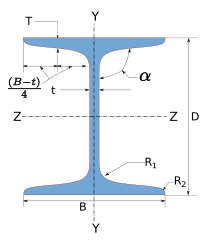
\includegraphics[width=5cm,height=5cm]{E:/office _anjali/columnspliceanjali/Osdag3/ResourceFiles/images/ISection.png}}&\multicolumn{2}{|c|}{Beam Section *}&\multicolumn{2}{|c|}{WPB 550x300x166.2}\\%
\cline{2%
-%
5}%
&\multicolumn{2}{|c|}{Preferences}&\multicolumn{2}{|c|}{Outside + Inside}\\%
\cline{2%
-%
5}%
&\multicolumn{2}{|c|}{Material *}&\multicolumn{2}{|c|}{E 250 (Fe 410 W)A}\\%
\cline{2%
-%
5}%
&\multicolumn{2}{|c|}{Ultimate strength, fu (MPa)}&\multicolumn{2}{|c|}{410}\\%
\cline{2%
-%
5}%
&Yield Strength , fy (MPa)&240&R1(mm)&2.7\\%
\cline{2%
-%
5}%
&Mass&166.23&R2(mm)&0.0\\%
\cline{2%
-%
5}%
&Area(mm2) {-} A&21180.0&Iz(mm4)&1119322000.0\\%
\cline{2%
-%
5}%
&D(mm)&540.0&Iy(mm4)&108122200.0\\%
\cline{2%
-%
5}%
&B(mm)&300.0&rz(mm)&229.9\\%
\cline{2%
-%
5}%
&t(mm)&12.5&ry(mm)&71.5\\%
\cline{2%
-%
5}%
&T(mm)&24.0&Zz(mm3)&4145640.0\\%
\cline{2%
-%
5}%
&FlangeSlope&90&Zy(mm3)&720810.0\\%
\cline{2%
-%
5}%
\hline%
\multicolumn{5}{|c|}{\textbf{Bolt Details}}\\%
\hline%
\hline%
\multicolumn{3}{|c|}{Diameter (mm)*}&\multicolumn{2}{|c|}{{[}12.0, 16.0, 20.0, 24.0, 30.0, 36.0{]}}\\%
\hline%
\hline%
\multicolumn{3}{|c|}{Grade *}&\multicolumn{2}{|c|}{{[}3.6, 4.6, 4.8, 5.6, 5.8, 6.8, 8.8, 9.8, 10.9, 12.9{]}}\\%
\hline%
\hline%
\multicolumn{3}{|c|}{Type *}&\multicolumn{2}{|c|}{Bearing Bolt}\\%
\hline%
\hline%
\multicolumn{3}{|c|}{Bolt hole type}&\multicolumn{2}{|c|}{Standard}\\%
\hline%
\hline%
\multicolumn{3}{|c|}{Slip factor (µ\_f)}&\multicolumn{2}{|c|}{0.3}\\%
\hline%
\hline%
\multicolumn{3}{|c|}{Type of edges}&\multicolumn{2}{|c|}{a {-} Sheared or hand flame cut}\\%
\hline%
\hline%
\multicolumn{3}{|c|}{Gap between beam and <br>support (mm)}&\multicolumn{2}{|c|}{10.0}\\%
\hline%
\hline%
\multicolumn{3}{|c|}{Are the members exposed to <br>corrosive influences}&\multicolumn{2}{|c|}{False}\\%
\hline%
\end{longtable}

%
\Needspace{10\baselineskip}%
\newpage%
\section{Design Checks}%
\label{sec:DesignChecks}%
\subsection{Member Capacity}%
\label{subsec:MemberCapacity}%
\renewcommand{\arraystretch}{1.2}%
\begin{longtable}{|p{4cm}|p{5cm}|p{5.5cm}|p{1.5cm}|}%
\hline%
\rowcolor{OsdagGreen}%
Check&Required&Provided&Remarks\\%
\hline%
\endhead%
\hline%
Axial Capacity Member Ac (kN)&&$\begin{aligned} A_c &=\frac{A*f_y}{\gamma_{m0} *10^3}\\ &=\frac{21180.0*240}{1.1* 10^3}\\ &=4621.09\end{aligned}$&\\%
\hline%
Shear Capacity Member Sc (kN)&&$\begin{aligned} S_c &= \frac{A_v*f_y}{\sqrt{3}*\gamma_{mo} *10^3}\\ &=\frac{492.0*12.5*240}{\sqrt{3}*1.1 *10^3}\\ &=774.7\end{aligned}$&\\%
\hline%
Plastic Moment Capacity Pmc (kNm)&&$\begin{aligned} Pmc &= \frac{\beta_b * Z_p *fy}{\gamma_{mo} * 10^6}\\ &=\frac{1*756450.0*240}{1.1 * 10^6}\\ &=165.04\end{aligned}$&\\%
\hline%
Moment Deformation Criteria Mdc (kNm)&&$\begin{aligned} Mdc &= \frac{1.5 *Z_e *fy}{1.1* 10^6}\\ &= \frac{1.5 *4145640.0*240}{1.1* 10^6}\\ &= 1356.75\end{aligned}$&\\%
\hline%
Moment Capacity Member Mc (kNm)&&$\begin{aligned} M_c &= min(Pmc,Mdc)\\ &=min(165.04,1356.75)\\ &=165.04\end{aligned}$&\\%
\hline%
\end{longtable}

%
\newpage%
\subsection{Load Consideration}%
\label{subsec:LoadConsideration}%
\renewcommand{\arraystretch}{1.2}%
\begin{longtable}{|p{4cm}|p{3.5cm}|p{6.5cm}|p{1.5cm}|}%
\hline%
\rowcolor{OsdagGreen}%
Check&Required&Provided&Remarks\\%
\hline%
\endhead%
\hline%
Applied Axial Load Au (kN)&$\begin{aligned} Ac_{min} &= 0.3 * A_c\\ &= 0.3 *4621.09\\ &=1386.33\\ Ac_{max} &= Ac \\ &=4621.09\end{aligned}$&$\begin{aligned} A_u &=1386.33\end{aligned}$&Pass\\%
\hline%
Applied Shear Load Vu (kN)&$\begin{aligned} Vc_{min} &= 0.6 * S_c\\ &= 0.6 *774.7\\ &=464.82\\ Vc_{max} &= Sc \\ &=774.7\end{aligned}$&$\begin{aligned} V_u &=464.82\end{aligned}$&Pass\\%
\hline%
Applied Moment Load Mu (kNm)&$\begin{aligned} Mc_{min} &= 0.5 * M_c\\ &= 0.5 *165.04\\ &=82.52\\  Mc_{max} &= Mc \\ &=165.04\end{aligned}$&$\begin{aligned} M_u &=82.52\end{aligned}$&Pass\\%
\hline%
Forces Carried by Web&&$\begin{aligned}A_w &= Axial~ force~ in~ web  \\   &= \frac{(D- 2*T)*t* Au }{A} \\ &= \frac{(540.0- 2*24.0)*12.5*1386.33 }{21180.0} \\ &=402.55~ kN\\ M_w &= Moment ~in ~web  \\  &= \frac{Z_w * Mu}{Z} \\ &= \frac{756450.0 * 82.52}{4621820.0} \\ &=13.51~{kNm}\end{aligned}$&\\%
\hline%
Forces Carried by Flange&&$\begin{aligned} A_f&= Axial~force~ in ~flange  \\ &= \frac{Au * B *T}{A} \\ &= \frac{1386.33 * 300.0*24.0}{21180.0} \\ &=471.27~ kN\\ M_f& =Moment~ in~ flange \\  & = Mu-M_w\\ &= 82.52-13.51\\ &=69.02~{kNm}\\  F_f& =flange~force  \\ & = \frac{M_f *10^3}{D-T} + A_f \\ &= \frac{69.02* 10^3}{540.0-24.0} +471.27 \\ &=605.02~kN \end{aligned}$&\\%
\hline%
\end{longtable}

%
\newpage%
\subsection{Initial Member Check}%
\label{subsec:InitialMemberCheck}%
\renewcommand{\arraystretch}{1.2}%
\begin{longtable}{|p{3cm}|p{4.5cm}|p{6.5cm}|p{1.5cm}|}%
\hline%
\rowcolor{OsdagGreen}%
Check&Required&Provided&Remarks\\%
\hline%
\endhead%
\hline%
Flange Tension Yielding Capacity (kN)&$\begin{aligned} F_f &=605.02\end{aligned}$&$\begin{aligned} T_{dg} &= \frac{l*t*f_y}{\gamma_{mo}}\\ &=\frac{1*300.0*24.0*240}{1.1}\\ &=1636.36\end{aligned}$&Pass\\%
\hline%
Web Tension Yielding Capacity (kN)&$\begin{aligned} A_w &=402.55\end{aligned}$&$\begin{aligned} T_{dg} &= \frac{l*t*f_y}{\gamma_{mo}}\\ &=\frac{1*492.0*12.5*240}{1.1}\\ &=1398\end{aligned}$&Pass\\%
\hline%
\end{longtable}

%
\newpage%
\subsection{Initial flange plate height check}%
\label{subsec:Initialflangeplateheightcheck}%
\renewcommand{\arraystretch}{1.2}%
\begin{longtable}{|p{4.5cm}|p{2.5cm}|p{7cm}|p{1.5cm}|}%
\hline%
\rowcolor{OsdagGreen}%
Check&Required&Provided&Remarks\\%
\hline%
\endhead%
\hline%
flange\_plate.Height&Outer.b >= 50&$\begin{aligned} Outer.b &=300.0\end{aligned}$&Pass\\%
\hline%
flange\_plate.InnerHeight&Inner.b >= 50&$\begin{aligned} inner.b &= \frac{B-t-(2*r_1)}{2}\\ &=\frac{300.0-12.5-(2*2.7)}{2}\\ &= 141.05\end{aligned}$&Pass\\%
\hline%
\end{longtable}

%
\newpage%
\subsection{Flange plate thickness}%
\label{subsec:Flangeplatethickness}%
\renewcommand{\arraystretch}{1.2}%
\begin{longtable}{|p{2.5cm}|p{4.5cm}|p{7cm}|p{1.5cm}|}%
\hline%
\rowcolor{OsdagGreen}%
Check&Required&Provided&Remarks\\%
\hline%
\endhead%
\hline%
Thickness (mm)*&$\begin{aligned} T &=12.0\end{aligned}$&$\begin{aligned} t_f &=14.0\end{aligned}$&Pass\\%
\hline%
Plate Area check (mm2)&$\begin{aligned} &pt.area >= \\&connected~member~area * 1.05\\  &= 7560.0\end{aligned}$&$\begin{aligned} outer.b &= B\\ &= 300.0 \\ inner.b &= \frac{B-t-(2*r_1)}{2}\\ &=\frac{300.0-12.5-(2*2.7)}{2}\\ &= 141.05 \\  pt.area &=(300.0+(2*141.05))*14.0\\ &= 8149.4\end{aligned}$&Pass\\%
\hline%
\end{longtable}

%
\newpage%
\subsection{Web plate thickness}%
\label{subsec:Webplatethickness}%
\renewcommand{\arraystretch}{1.2}%
\begin{longtable}{|p{2.5cm}|p{4.5cm}|p{7cm}|p{1.5cm}|}%
\hline%
\rowcolor{OsdagGreen}%
Check&Required&Provided&Remarks\\%
\hline%
\endhead%
\hline%
Thickness (mm)*&$\begin{aligned} t &=6.25\end{aligned}$&$\begin{aligned} t_w &=20.0\end{aligned}$&Pass\\%
\hline%
Plate Area check (mm2)&$\begin{aligned} &pt.area >= \\&connected~member~area * 1.05\\  &= 5827.5\end{aligned}$&$\begin{aligned} web~b &= D-(2*T)-(2*r_1)\\ &=540.0-(2*24.0)-(2*2.7)\\ &= 444.0 \\  pt.area &= 20.0*2* 444.0\\ &= 17760.0\end{aligned}$&Pass\\%
\hline%
\end{longtable}

%
\newpage%
\subsection{Web Spacing Checks}%
\label{subsec:WebSpacingChecks}%
\renewcommand{\arraystretch}{1.2}%
\begin{longtable}{|p{2.5cm}|p{7.5cm}|p{5cm}|p{1cm}|}%
\hline%
\rowcolor{OsdagGreen}%
Check&Required&Provided&Remarks\\%
\hline%
\endhead%
\hline%
Min.Diameter (mm)&&$\begin{aligned} d &=12.0\end{aligned}$&\\%
\hline%
Min. Gauge (mm)&$\begin{aligned}p/g_{min}&= 2.5 ~ d&\\ =&2.5*12.0&=30.0\end{aligned}$&$\begin{aligned} g &=90~(Row~Limit~(r_l) = 2)\end{aligned}$&\\%
\hline%
Min. Edge Distance (mm)&$\begin{aligned}e/e`_{min} &=[1.5~or~ 1.7] * d_0\\ &=1.7*13.0=22.1 \end{aligned}$&70&\\%
\hline%
Spacing Check&$\begin{aligned} depth & = 2 * e + (r_l -1) * g\\ & = 2 * 70+(2.0-1)*90\\ & = 230.0\end{aligned}$&444.0&Pass\\%
\hline%
\end{longtable}

%
\newpage%
\subsection{Flange Spacing Checks}%
\label{subsec:FlangeSpacingChecks}%
\renewcommand{\arraystretch}{1.2}%
\begin{longtable}{|p{2.5cm}|p{7.5cm}|p{5cm}|p{1cm}|}%
\hline%
\rowcolor{OsdagGreen}%
Check&Required&Provided&Remarks\\%
\hline%
\endhead%
\hline%
Min.Diameter (mm)&&$\begin{aligned} d &=12.0\end{aligned}$&\\%
\hline%
Min. Gauge (mm)&$\begin{aligned}p/g_{min}&= 2.5 ~ d&\\ =&2.5*12.0&=30.0\end{aligned}$&$\begin{aligned} g &=0.0~(Row~Limit~(r_l) = 1)\end{aligned}$&\\%
\hline%
Min. Edge Distance (mm)&$\begin{aligned}e/e`_{min} &=[1.5~or~ 1.7] * d_0\\ &=1.7*13.0=22.1 \end{aligned}$&70&\\%
\hline%
Spacing Check&$\begin{aligned} depth & = 2 * e + (r_l -1) * g\\ & = 2 * 70+(1.0-1)*90\\ & = 140.0\end{aligned}$&141.05&Pass\\%
\hline%
\end{longtable}

%
\newpage%
\subsection{Flange Bolt Checks}%
\label{subsec:FlangeBoltChecks}%
\renewcommand{\arraystretch}{1.2}%
\begin{longtable}{|p{4cm}|p{5cm}|p{5.5cm}|p{1.5cm}|}%
\hline%
\rowcolor{OsdagGreen}%
Check&Required&Provided&Remarks\\%
\hline%
\endhead%
\hline%
Diameter (mm)&Bolt Quantity Optimisation&$\begin{aligned} d &=36.0\end{aligned}$&\\%
\hline%
Grade&Bolt Grade Optimisation&3.6&\\%
\hline%
Bolt.fu&&300.0&\\%
\hline%
Bolt.fy&&180.0&\\%
\hline%
Hole Diameter (mm)& &$\begin{aligned} d_0 &=39.0\end{aligned}$&\\%
\hline%
Shear Capacity (kN)&&$\begin{aligned}V_{dsb} &= \frac{f_{ub} ~n_n~ A_{nb}}{\sqrt{3} ~\gamma_{mb}}\\ &= \frac{300.0*2*817}{\sqrt{3}~*~1.25}\\ &= 226.41\end{aligned}$&\\%
\hline%
Bearing Capacity (kN)&&$\begin{aligned}V_{dpb} &= \frac{2.5~ k_b~ d~ t~ f_u}{\gamma_{mb}}\\ &= \frac{2.5~*0.52*36.0*24.0*410}{1.25}\\ &=368.41\end{aligned}$&\\%
\hline%
Bolt Capacity (kN)&&$\begin{aligned}V_{db} &= min~ (V_{dsb}, V_{dpb})\\ &= min~ (226.41,368.41)\\ &=226.41\end{aligned}$&\\%
\hline%
No of Bolts&$\begin{aligned}R_{u} &= \sqrt{V_u^2+A_u^2}\\ n_{trial} &= R_u/ V_{bolt}\\ R_{u} &= \frac{\sqrt{0.0^2+605.02^2}}{226.41}\\ &=6\end{aligned}$&8&\\%
\hline%
No of Columns&&$\begin{aligned} n_c &=4\end{aligned}$&\\%
\hline%
No of Rows&&$\begin{aligned} n_r &=2\end{aligned}$&\\%
\hline%
Min. Pitch (mm)&$\begin{aligned}p/g_{min}&= 2.5 ~ d&\\ =&2.5*36.0&=90.0\end{aligned}$&90&Pass\\%
\hline%
Max. Pitch (mm)&$\begin{aligned}p/g_{max} &=\min(32~t,~300~mm)&\\ &=\min(32 *~14.0,~ 300 ~mm)\\&=300\end{aligned}$&90&Pass\\%
\hline%
Min. Gauge (mm)&$\begin{aligned}p/g_{min}&= 2.5 ~ d&\\ =&2.5*36.0&=90.0\end{aligned}$&0.0&N/A\\%
\hline%
Max. Gauge (mm)&$\begin{aligned}p/g_{max} &=\min(32~t,~300~mm)&\\ &=\min(32 *~14.0,~ 300 ~mm)\\&=300\end{aligned}$&0.0&N/A\\%
\hline%
Min. End Distance (mm)&$\begin{aligned}e/e`_{min} &=[1.5~or~ 1.7] * d_0\\ &=1.7*39.0=66.3 \end{aligned}$&70&Pass\\%
\hline%
Max. End Distance (mm)&$\begin{aligned}e/e`_{max} &= 12~ t~ \varepsilon&\\ \varepsilon &= \sqrt{\frac{250}{f_y}}\\ e/e`_{max}&=12 ~*14.0*\sqrt{\frac{250}{250}}\\ &=168.0\\ \end{aligned}$&70&Pass\\%
\hline%
Min. Edge Distance (mm)&$\begin{aligned}e/e`_{min} &=[1.5~or~ 1.7] * d_0\\ &=1.7*39.0=66.3 \end{aligned}$&70.525&Pass\\%
\hline%
Max. Edge Distance (mm)&$\begin{aligned}e/e`_{max} &= 12~ t~ \varepsilon&\\ \varepsilon &= \sqrt{\frac{250}{f_y}}\\ e/e`_{max}&=12 ~*14.0*\sqrt{\frac{250}{250}}\\ &=168.0\\ \end{aligned}$&70.525&Pass\\%
\hline%
Bolt Capacity post Long Joint (kN)&$\begin{aligned} &if~l\geq 15 * d~then~V_{rd} = \beta_{ij} * V_{db} \\ & if~l < 15 * d~then~V_{rd} = V_{db} \\ & where,\\ & l = ((nc~or~nr) - 1) * (p~or~g) \\ & \beta_{ij} = 1.075 - l/(200 * d) \\ & but~0.75\leq\beta_{ij}\leq1.0 \end{aligned}$&$\begin{aligned} l~&= ((nc~or~nr) - 1) * (p~or~g) \\  lc&= 2*((\frac{4}{2} - 1) * 90+70)+ 10.0\\&=330.0\\  lr&= 2*((\frac{2}{2} - 1) * 0.0+70.525\\& +2.7)+ 12.5=158.95000000000002\\  l~&= 330.0\\ & 15 * d = 15 * 36.0 = 540.0 \\ & since,~l < 15 * d~ \\& then~V_{rd} = V_{db} \\ & V_{rd} = 226.41 \end{aligned}$&\\%
\hline%
Capacity (kN)&151.26&226.41&Pass\\%
\hline%
\end{longtable}

%
\newpage%
\subsection{Web Bolt Checks}%
\label{subsec:WebBoltChecks}%
\renewcommand{\arraystretch}{1.2}%
\begin{longtable}{|p{4cm}|p{5cm}|p{5.5cm}|p{1.5cm}|}%
\hline%
\rowcolor{OsdagGreen}%
Check&Required&Provided&Remarks\\%
\hline%
\endhead%
\hline%
Shear Capacity (kN)&&$\begin{aligned}V_{dsb} &= \frac{f_{ub} ~n_n~ A_{nb}}{\sqrt{3} ~\gamma_{mb}}\\ &= \frac{300.0*2*817}{\sqrt{3}~*~1.25}\\ &= 226.41\end{aligned}$&\\%
\hline%
Bearing Capacity (kN)&&$\begin{aligned}V_{dpb} &= \frac{2.5~ k_b~ d~ t~ f_u}{\gamma_{mb}}\\ &= \frac{2.5~*0.52*36.0*12.5*410}{1.25}\\ &=191.88\end{aligned}$&\\%
\hline%
Bolt Capacity (kN)&&$\begin{aligned}V_{db} &= min~ (V_{dsb}, V_{dpb})\\ &= min~ (226.41,191.88)\\ &=191.88\end{aligned}$&\\%
\hline%
No of Bolts&$\begin{aligned}R_{u} &= \sqrt{V_u^2+A_u^2}\\ n_{trial} &= R_u/ V_{bolt}\\ R_{u} &= \frac{\sqrt{464.82^2+402.55^2}}{191.88}\\ &=8\end{aligned}$&16&\\%
\hline%
No of Columns&&$\begin{aligned} n_c &=4\end{aligned}$&\\%
\hline%
No of Rows&&$\begin{aligned} n_r &=4\end{aligned}$&\\%
\hline%
Min. Pitch (mm)&$\begin{aligned}p/g_{min}&= 2.5 ~ d&\\ =&2.5*36.0&=90.0\end{aligned}$&90&Pass\\%
\hline%
Max. Pitch (mm)&$\begin{aligned}p/g_{max} &=\min(32~t,~300~mm)&\\ &=\min(32 *~12.5,~ 300 ~mm)\\&=300\end{aligned}$&90&Pass\\%
\hline%
Min. Gauge (mm)&$\begin{aligned}p/g_{min}&= 2.5 ~ d&\\ =&2.5*36.0&=90.0\end{aligned}$&90&Pass\\%
\hline%
Max. Gauge (mm)&$\begin{aligned}p/g_{max} &=\min(32~t,~300~mm)&\\ &=\min(32 *~12.5,~ 300 ~mm)\\&=300\end{aligned}$&90&Pass\\%
\hline%
Min. End Distance (mm)&$\begin{aligned}e/e`_{min} &=[1.5~or~ 1.7] * d_0\\ &=1.7*39.0=66.3 \end{aligned}$&70&Pass\\%
\hline%
Max. End Distance (mm)&$\begin{aligned}e/e`_{max} &= 12~ t~ \varepsilon&\\ \varepsilon &= \sqrt{\frac{250}{f_y}}\\ e/e`_{max}&=12 ~*20.0*\sqrt{\frac{250}{250}}\\ &=240.0\\ \end{aligned}$&70&Pass\\%
\hline%
Min. Edge Distance (mm)&$\begin{aligned}e/e`_{min} &=[1.5~or~ 1.7] * d_0\\ &=1.7*39.0=66.3 \end{aligned}$&70&Pass\\%
\hline%
Max. Edge Distance (mm)&$\begin{aligned}e/e`_{max} &= 12~ t~ \varepsilon&\\ \varepsilon &= \sqrt{\frac{250}{f_y}}\\ e/e`_{max}&=12 ~*20.0*\sqrt{\frac{250}{250}}\\ &=240.0\\ \end{aligned}$&70&Pass\\%
\hline%
Parameters required for bolt force (mm)&&$\begin{aligned} l_n~~~ &= length~available \\  l_n~~~ &= (n_r - 1) * g\\  &= (4 - 1) *90\\  & =270\\  y_{max} &= l_n / 2\\  &= 270 / 2 \\  & =135.0\\ x_{max} &= p * (\frac{n_c}{2} - 1) / 2 \\  &= 90 * (\frac{4}{2} + - 1) / 2 \\  & =45.0\end{aligned}$&\\%
\hline%
Moment Demand (kNm&&$\begin{aligned}  M_d &= (V_u * ecc + M_w)\\  &= \frac{(464.82 * 10^3 *120.0 + 13.51*10^6)}{10^6}\\  & =69.28\end{aligned}$&\\%
\hline%
Bolt.Force&&$\begin{aligned} vbv~~ &= V_u / (n_r * n_c)\\  &= \frac{464.82}{ (4*4)}\\  & =58.1\\ tmh~ &= \frac{M_d * y_{max} }{ \Sigma r_i^2} \\  &= \frac{69.28 *135.0}{97.2}\\  & =96.23\\  tmv ~&= \frac{M_d * x_{max}}{\Sigma r_i^2}\\ &= \frac{69.28 * 45.0}{97.2}\\  & =32.08\\  abh~ & = \frac{A_u }{(n_r * n_c)}\\   & =\frac{402.55}{ (4 *4)}\\  & =50.32\\  vres &=\sqrt{(vbv +tmv) ^ 2 + (tmh+abh) ^ 2}\\   &= \sqrt{(58.1 +32.08) ^2 + (96.23+50.32) ^ 2}\\  & =172.07\end{aligned}$&\\%
\hline%
Bolt Capacity post Long Joint (kN)&$\begin{aligned} &if~l\geq 15 * d~then~V_{rd} = \beta_{ij} * V_{db} \\ & if~l < 15 * d~then~V_{rd} = V_{db} \\ & where,\\ & l = ((nc~or~nr) - 1) * (p~or~g) \\ & \beta_{ij} = 1.075 - l/(200 * d) \\ & but~0.75\leq\beta_{ij}\leq1.0 \end{aligned}$&$\begin{aligned} l&= ((nc~or~nr) - 1) * (p~or~g) \\  lc&= 2*((\frac{4}{2} - 1) * 90+70)+ 10.0\\&=330.0\\  lr&= (4 - 1) * 90=270\\  l&= 330.0\\ & 15 * d = 15 * 36.0 = 540.0 \\ & since,~l < 15 * d~\\&then~V_{rd} = V_{db} \\ & V_{rd} = 191.88 \end{aligned}$&\\%
\hline%
Capacity (kN)&172.07&191.88&Pass\\%
\hline%
\end{longtable}

%
\newpage%
\subsection{Inner and Outer flange plate Checks}%
\label{subsec:InnerandOuterflangeplateChecks}%
\renewcommand{\arraystretch}{1.2}%
\begin{longtable}{|p{4cm}|p{6cm}|p{5.5cm}|p{1.5cm}|}%
\hline%
\rowcolor{OsdagGreen}%
Check&Required&Provided&Remarks\\%
\hline%
\endhead%
\hline%
Min. Plate Height (mm)&$\begin{aligned}min~flange~plate~ht &= beam~width\\ &=300.0\end{aligned}$&300.0&Pass\\%
\hline%
Min. Plate Length (mm)&$\begin{aligned} & 2[2*e_{min} + ({\frac{bolt~lines}{2}}-1) * p_{min})]\\ & +\frac{gap}{2}]\\ &=2*[(2*66.3 + (\frac{4}{2}-1) * 90.0\\ &= + \frac{10.0}{2}]\\ &=455.2\end{aligned}$&470.0&Pass\\%
\hline%
Min. Inner Plate Height (mm)&$\begin{aligned}&= \frac{B -t- (2*R1)}{2}\\ &=\frac{300.0 -12.5 - 2*2.7}{2}\\ &=141.05\end{aligned}$&141.05&Pass\\%
\hline%
Max. Inner Plate Height (mm)&$\begin{aligned}&= \frac{B -t- (2*R1)}{2}\\ &=\frac{300.0 -12.5 - 2*2.7}{2}\\ &=141.05\end{aligned}$&141.05&Pass\\%
\hline%
Min. Inner Plate Length (mm)&$\begin{aligned} & 2[2*e_{min} + ({\frac{bolt~lines}{2}}-1) * p_{min})]\\ & +\frac{gap}{2}]\\ &=2*[(2*66.3 + (\frac{4}{2}-1) * 90.0\\ &= + \frac{10.0}{2}]\\ &=455.2\end{aligned}$&470.0&Pass\\%
\hline%
Min.Plate Thickness (mm)&$\begin{aligned} t_w=12.0\end{aligned}$&14.0&Pass\\%
\hline%
\end{longtable}

%
\newpage%
\subsection{Member Checks}%
\label{subsec:MemberChecks}%
\renewcommand{\arraystretch}{1.2}%
\begin{longtable}{|p{4cm}|p{6cm}|p{5.5cm}|p{1.5cm}|}%
\hline%
\rowcolor{OsdagGreen}%
Check&Required&Provided&Remarks\\%
\hline%
\endhead%
\hline%
Flange Tension Yielding Capacity (kN)&&$\begin{aligned} T_{dg} &= \frac{l*t*f_y}{\gamma_{mo}}\\ &=\frac{1*300.0*24.0*240}{1.1}\\ &=1636.36\end{aligned}$&\\%
\hline%
Flange Tension Rupture Capacity (kN)&&$\begin{aligned} T_{dn} &= \frac{0.9*A_{n}*f_u}{\gamma_{m1}}\\ &=\frac{0.9*(300.0-2*39.0)*24.0*410}{1.25}\\ &=1572.83\end{aligned}$&\\%
\hline%
Flange Block Shear Capacity (kN)&&$\begin{aligned}T_{db1} &= \frac{A_{vg} f_{y}}{\sqrt{3} \gamma_{m0}} + \frac{0.9 A_{tn} f_{u}}{\gamma_{m1}}\\ T_{db2} &= \frac{0.9*A_{vn} f_{u}}{\sqrt{3} \gamma_{m1}} + \frac{A_{tg} f_{y}}{\gamma_{m0}}\\ T_{db} &= min(T_{db1}, T_{db2})= 1599.72\end{aligned}$&\\%
\hline%
Flange Tension Capacity (kN)&$\begin{aligned} f_f &=605.02\end{aligned}$&$\begin{aligned} T_d &= min(T_{dg},T_{dn},T_{db})\\ &= min(1636.36,1572.83,1599.72)\\ &=1572.83\end{aligned}$&Pass\\%
\hline%
Web Tension Yielding Capacity (kN)&&$\begin{aligned} T_{dg} &= \frac{l*t*f_y}{\gamma_{mo}}\\ &=\frac{1*492.0*12.5*240}{1.1}\\ &=1397.73\end{aligned}$&\\%
\hline%
Web Tension Rupture Capacity (kN)&&$\begin{aligned} T_{dn} &= \frac{0.9*A_{n}*f_u}{\gamma_{m1}}\\ &=\frac{0.9*(492.0-4*39.0)*12.5*410}{1.25}\\ &=1239.84\end{aligned}$&\\%
\hline%
Web Block Shear Capacity (kN)&&$\begin{aligned}T_{db1} &= \frac{A_{vg} f_{y}}{\sqrt{3} \gamma_{m0}} + \frac{0.9 A_{tn} f_{u}}{\gamma_{m1}}\\ T_{db2} &= \frac{0.9*A_{vn} f_{u}}{\sqrt{3} \gamma_{m1}} + \frac{A_{tg} f_{y}}{\gamma_{m0}}\\ T_{db} &= min(T_{db1}, T_{db2})= 1347.73\end{aligned}$&\\%
\hline%
Web Tension Capacity (kN)&$\begin{aligned} A_w &=402.55\end{aligned}$&$\begin{aligned} T_d &= min(T_{dg},T_{dn},T_{db})\\ &= min(1397.73,1239.84,1347.73)\\ &=1239.84\end{aligned}$&Pass\\%
\hline%
\end{longtable}

%
\newpage%
\subsection{Flange Plate Capacity Checks in axial{-}Outside/Inside }%
\label{subsec:FlangePlateCapacityChecksinaxial{-}Outside/Inside}%
\renewcommand{\arraystretch}{1.2}%
\begin{longtable}{|p{4cm}|p{6cm}|p{5.5cm}|p{1.5cm}|}%
\hline%
\rowcolor{OsdagGreen}%
Check&Required&Provided&Remarks\\%
\hline%
\endhead%
\hline%
Tension Yielding Capacity (kN)&&$\begin{aligned} T_{dg} &= \frac{l*t*f_y}{\gamma_{mo}}\\ &=\frac{1*582.1*14.0*250}{1.1}\\ &=1852.14\end{aligned}$&\\%
\hline%
Tension Rupture Capacity (kN)&&$\begin{aligned} T_{dn} &= \frac{0.9*A_{n}*f_u}{\gamma_{m1}}\\ &=\frac{0.9*(582.1-2*39.0)*14.0*410}{1.25}\\ &=2083.34\end{aligned}$&\\%
\hline%
Block Shear Capacity (kN)&&$\begin{aligned}T_{db1} &= \frac{A_{vg} f_{y}}{\sqrt{3} \gamma_{m0}} + \frac{0.9 A_{tn} f_{u}}{\gamma_{m1}}\\ T_{db2} &= \frac{0.9*A_{vn} f_{u}}{\sqrt{3} \gamma_{m1}} + \frac{A_{tg} f_{y}}{\gamma_{m0}}\\ T_{db} &= min(T_{db1}, T_{db2})= 1923.29\end{aligned}$&\\%
\hline%
Plate Tension Capacity (kN)&$\begin{aligned} f_f &=605.02\end{aligned}$&$\begin{aligned} T_d &= min(T_{dg},T_{dn},T_{db})\\ &= min(1852.14,2083.34,1923.29)\\ &=1852.14\end{aligned}$&Pass\\%
\hline%
\end{longtable}

%
\newpage%
\subsection{Web Plate Capacity Checks in Axial}%
\label{subsec:WebPlateCapacityChecksinAxial}%
\renewcommand{\arraystretch}{1.2}%
\begin{longtable}{|p{4cm}|p{6cm}|p{5.5cm}|p{1.5cm}|}%
\hline%
\rowcolor{OsdagGreen}%
Check&Required&Provided&Remarks\\%
\hline%
\endhead%
\hline%
Tension Yielding Capacity (kN)&&$\begin{aligned} T_{dg} &= \frac{l*t*f_y}{\gamma_{mo}}\\ &=\frac{1*410*20.0*250}{1.1}\\ &=2151.94\end{aligned}$&\\%
\hline%
Tension Rupture Capacity (kN)&&$\begin{aligned} T_{dn} &= \frac{0.9*A_{n}*f_u}{\gamma_{m1}}\\ &=\frac{0.9*(410-4*39.0)*20.0*300.0}{1.25}\\ &=2999.23\end{aligned}$&\\%
\hline%
Block Shear Capacity (kN)&&$\begin{aligned}T_{db1} &= \frac{A_{vg} f_{y}}{\sqrt{3} \gamma_{m0}} + \frac{0.9 A_{tn} f_{u}}{\gamma_{m1}}\\ T_{db2} &= \frac{0.9*A_{vn} f_{u}}{\sqrt{3} \gamma_{m1}} + \frac{A_{tg} f_{y}}{\gamma_{m0}}\\ T_{db} &= min(T_{db1}, T_{db2})= 4312.75\end{aligned}$&\\%
\hline%
Plate Tension Capacity (kN)&$\begin{aligned} A_w &=402.55\end{aligned}$&$\begin{aligned} T_d &= min(T_{dg},T_{dn},T_{db})\\ &= min(3727.27,2999.23,4312.75)\\ &=2999.23\end{aligned}$&Pass\\%
\hline%
\end{longtable}

%
\newpage%
\subsection{Web Plate Capacity Checks in Shear}%
\label{subsec:WebPlateCapacityChecksinShear}%
\renewcommand{\arraystretch}{1.2}%
\begin{longtable}{|p{4cm}|p{6cm}|p{5.5cm}|p{1.5cm}|}%
\hline%
\rowcolor{OsdagGreen}%
Check&Required&Provided&Remarks\\%
\hline%
\endhead%
\hline%
Shear yielding Capacity (V\_dy) (kN)&&$\begin{aligned} V_{dy} &= \frac{A_v*f_y}{\sqrt{3}*\gamma_{mo}}\\ &=\frac{1*410*20.0*250}{\sqrt{3}*1.1}\\ &=2151.94\end{aligned}$&\\%
\hline%
Shear Rupture Capacity (V\_dn) (kN)&&$\begin{aligned} V_{dn} &= \frac{0.9*A_{vn}*f_u}{\sqrt{3}*\gamma_{m1}}\\ &= \frac{0.9 *(410-(2.0*39.0))*20.0*410}{\sqrt{3}*1.25}\\ &=1731.61\end{aligned}$&\\%
\hline%
Block Shear Capacity in Shear (V\_db) (kN)&&$\begin{aligned}T_{db1} &= \frac{A_{vg} f_{y}}{\sqrt{3} \gamma_{m0}} + \frac{0.9 A_{tn} f_{u}}{\gamma_{m1}}\\ T_{db2} &= \frac{0.9*A_{vn} f_{u}}{\sqrt{3} \gamma_{m1}} + \frac{A_{tg} f_{y}}{\gamma_{m0}}\\ T_{db} &= min(T_{db1}, T_{db2})= 2841.88\end{aligned}$&\\%
\hline%
Plate Shear Capacity (kN)&$\begin{aligned} V_u &=464.82\end{aligned}$&$\begin{aligned} V_d &= min(V_{dy},V_{dn},V_{db})\\ &= min(2151.94,1731.61,4312.75)\\ &=1731.61\end{aligned}$&Pass\\%
\hline%
\end{longtable}

%
\Needspace{10\baselineskip}%
\newpage%
\section{3D View}%
\label{sec:3DView}%


\begin{figure}[h!]%
\centering%
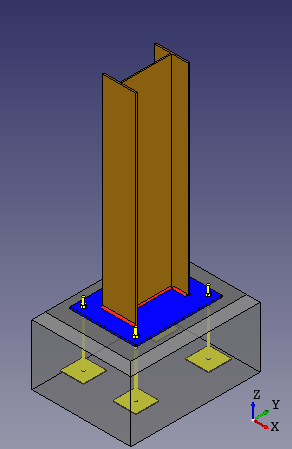
\includegraphics[width=\linewidth]{E:/office _anjali/columnspliceanjali/Osdag3/ResourceFiles/images/3d.png}%
\caption{3D View}%
\end{figure}

%
\end{document}